% Chapter 2

\chapter{Preliminary results and Future Work} % Write in your own chapter title
\label{Chapter3}
\lhead{\emph{Preliminary results and Future Work}} % Write in your own chapter title to set the page header
\fancyfoot[CE,CO]{\hline \\ \small Alshaima Alnaqbi  • Dep. of Applied Physics and Astronomy • UoS • 2026}

This chapter presents the preliminary results obtained from dynamic single-zone nuclear reaction network calculations of nova hydrogen burning. Two thermodynamic prescriptions were considered. The first is an exponential expansion model, in which the temperature and density decrease analytically with time. The second is a thermodynamic trajectory model, in which the temperature and density are taken from an external nova trajectory profile.

The main diagnostic quantity used to compare the two calculations is the CNO isotopic ratio (Equation~\ref{eq:ratio}). This ratio traces the redistribution of material between the $A=14$ and $A=15$ CNO isotopes during hydrogen burning. It is particularly useful because it is sensitive to proton captures, beta decays, and freeze-out during the hot-CNO cycle.

The preliminary calculations show that the final value of $R_{15/14}$ is strongly affected by the adopted thermodynamic history. The exponential model produces rapid early burning followed by freeze-out, while the trajectory model produces a stronger enhancement because of a delayed temperature peak. These results provide the basis for the future work described later in this chapter, which will include larger nuclear networks, reaction-flow analysis, timescale calculations, and quasi-equilibrium diagnostics.

\section{Exponential Single-Zone Calculation}

\subsection{Thermodynamic Evolution}

The preliminary exponential calculation was performed using $T_{9,0}=0.20, \rho_0 = 1.5\times10^4~\mathrm{g~cm^{-3}},\\ \tau = 0.2~\mathrm{s},$ and $t_{\mathrm{end}} = 100~\mathrm{s}$. Under these conditions, the temperature and density decrease rapidly at early times. The temperature begins at $T_9=0.20$ and falls monotonically as the material expands. As a result, the nuclear reaction rates are largest at the beginning of the calculation and then decline quickly as the system cools. This behaviour leads to an early phase of active hydrogen burning followed by freeze-out, when the temperature becomes too low for further efficient nuclear processing.

\begin{figure}[h!]
    \centering
    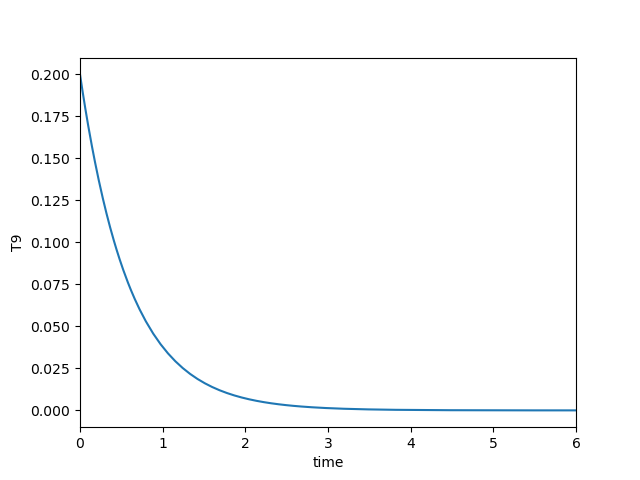
\includegraphics[width=0.75\textwidth]{Figures/Figure_1_exp.png}
    \caption{Temperature evolution for the exponential single-zone calculation. The temperature decreases rapidly from the initial value because of the imposed exponential expansion.}
    \label{fig:exp_t9}
\end{figure}

\subsection{Evolution of the CNO Diagnostic Ratio}

The abundance ratio (Equation~\ref{eq:ratio}) was calculated throughout the simulation. The initial value of this ratio is close to the solar-composition value. From the initial abundances, $X(^{14}\mathrm{N}) \simeq 7.97\times10^{-4}, X(^{15}\mathrm{N}) \simeq 3.14\times10^{-6}$, while the initial $^{14}\mathrm{O}$ and $^{15}\mathrm{O}$ abundances are very small. Therefore, the initial value of the ratio is approximately
\[
R_{15/14}^{\mathrm{initial}}
\approx
\frac{3.14\times10^{-6}}{7.97\times10^{-4}}
\approx 3.9\times10^{-3}.
\]

The calculation shows that $R_{15/14}$ first changes during the early active burning phase and then increases strongly before reaching a nearly constant freeze-out value. The final plateau is approximately
\[
R_{15/14}^{\mathrm{final}} \approx 0.4-0.5.
\]
This corresponds to an enhancement factor of roughly
\[
f_{\mathrm{enh}}
=
\frac{R_{15/14}^{\mathrm{final}}}
{R_{15/14}^{\mathrm{initial}}}
\sim 100.
\]

This result indicates that the exponential expansion model produces a significant enhancement of $^{15}\mathrm{N}$-rich material relative to the initial composition. The enhancement occurs because nuclear burning modifies the CNO isotopic distribution before the system cools and freezes out.

\begin{figure}[h!]
    \centering
    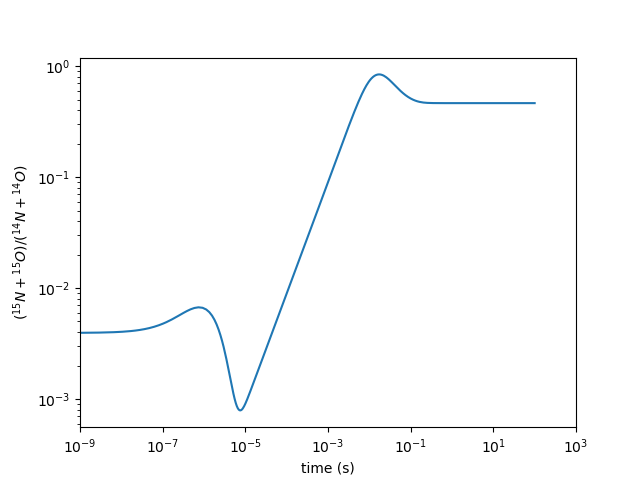
\includegraphics[width=0.75\textwidth]{Figures/Figure_2_exp.png}
    \caption{Evolution of the diagnostic abundance ratio $R_{15/14}$ for the exponential single-zone calculation. The ratio increases by about two orders of magnitude before reaching a freeze-out plateau.}
    \label{fig:exp_ratio}
\end{figure}

\section{Thermodynamic Trajectory Single-Zone Calculation}

\subsection{Trajectory Temperature and Density Evolution}

In the trajectory-based calculation, the temperature and density are not prescribed by a simple analytic function. Instead, they are read from a nova thermodynamic trajectory file. The calculation begins at a lower temperature than the exponential case and then follows a more complex nova-like evolution.

The trajectory begins near $T_9 \approx 0.091$, with a density of approximately $\rho \approx 2.21\times10^4~\mathrm{g~cm^{-3}}$. 
The temperature remains low during the early part of the calculation, then rises sharply and reaches a delayed maximum. After this peak, the temperature decreases again, and the nuclear reactions eventually freeze out.

This thermodynamic behaviour is very different from the exponential case. In the exponential calculation, the system begins hot and cools immediately. In the trajectory calculation, the system begins cooler, evolves for some time, and then experiences a strong heating phase. This delayed heating allows nuclear reactions to proceed under different conditions and produces a different final abundance pattern.

\begin{figure}[h!]
    \centering
    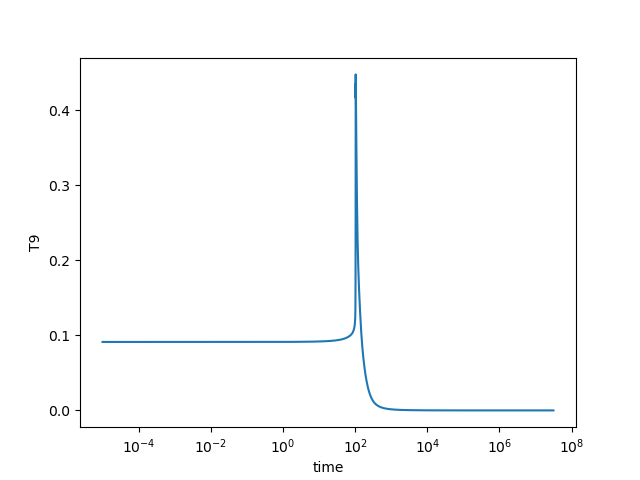
\includegraphics[width=0.75\textwidth]{Figures/Figure_1_traj.png}
    \caption{Temperature evolution for the trajectory-based single-zone calculation. The trajectory begins at relatively low temperature, later reaches a delayed temperature peak, and then cools toward freeze-out.}
    \label{fig:traj_t9}
\end{figure}

\subsection{Evolution of the CNO Diagnostic Ratio}

The same diagnostic ratio was calculated for the trajectory-based model. As in the exponential case, the initial value is close to
$ R_{15/14}^{\mathrm{initial}} \approx 4\times10^{-3}.$ During the early low-temperature phase, the ratio changes only slowly. As the trajectory approaches the temperature peak, proton-capture reactions become more efficient, and the hot-CNO reaction flow becomes stronger. This leads to a rapid modification of the $A=14$ and $A=15$ CNO abundances. After the temperature decreases, the reaction rates become too slow to maintain active burning, and the ratio reaches a final freeze-out plateau.

The final value of the ratio in the trajectory model is significantly larger than in the exponential model. The preliminary results show that $R_{15/14}^{\mathrm{final}}$ reaches a value of order a few. This means that the trajectory model produces a stronger enhancement of $^{15}\mathrm{N}$-rich material than the exponential model.

\begin{figure}[h!]
    \centering
    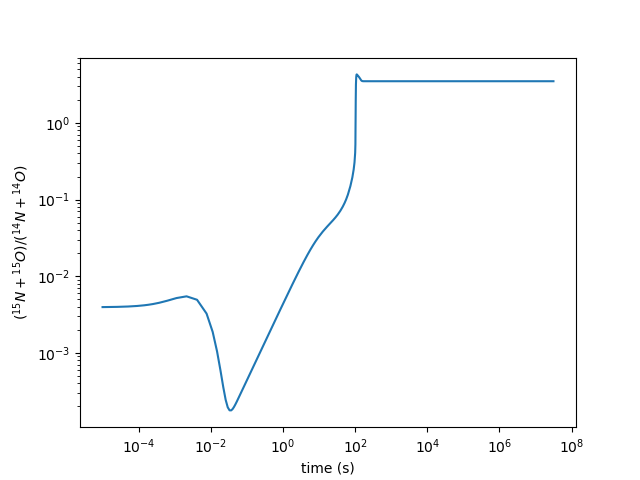
\includegraphics[width=0.75\textwidth]{Figures/Figure_2_traj.png}
    \caption{Evolution of the diagnostic abundance ratio $R_{15/14}$ for the trajectory-based single-zone calculation. The delayed temperature peak produces stronger hot-CNO processing and a larger final enhancement than in the exponential model.}
    \label{fig:traj_ratio}
\end{figure}

\section{Comparison Between the Exponential and Trajectory Calculations}

The two preliminary calculations demonstrate that the adopted thermodynamic history has a major effect on the final CNO isotopic composition. In the exponential case, the temperature starts at $T_9=0.20$ and decreases immediately. Therefore, most nuclear processing occurs at early times, and the abundance pattern freezes out rapidly. In contrast, the trajectory calculation begins at a lower temperature but later reaches a delayed temperature peak. This delayed heating phase allows stronger hot-CNO processing before freeze-out.

The most important difference is seen in the final value of the diagnostic ratio $R_{15/14}$. In the exponential model, the final value is approximately $R_{15/14}^{\mathrm{final}} \approx 0.4-0.5$, while in the trajectory model it reaches a value of order a few. Therefore, the trajectory model produces a stronger enhancement of $^{15}\mathrm{N}+^{15}\mathrm{O}$ relative to $^{14}\mathrm{N}+^{14}\mathrm{O}$.

\begin{table}[h!]
\centering
\caption{Summary of preliminary single-zone results.}
\begin{tabular}{llll}
\hline
Model & Thermodynamic behavior & Final $R_{15/14}$ & Interpretation \\
\hline
Exponential & Immediate cooling & $\sim 0.4-0.5$ & Early burning and freeze-out \\
Trajectory & Delayed temperature peak & order of a few & Stronger hot-CNO processing \\
\hline
\end{tabular}
\label{tab:preliminary_results}
\end{table}

These preliminary results suggest that the shape of the temperature-density history is not a minor detail. It directly affects the balance between proton captures, beta decays, and freeze-out. Therefore, realistic thermodynamic trajectories are essential for interpreting nova hydrogen burning and CNO isotope production.

\section{Physical Interpretation of the Preliminary Results}

The enhancement of $R_{15/14}$ can be understood as the result of competition between nuclear production and destruction channels in the hot-CNO cycle. Important reactions include $^{14}\mathrm{N}(p,\gamma)^{15}\mathrm{O}, ^{15}\mathrm{O}(\beta^+)^{15}\mathrm{N}, ^{15}\mathrm{N}(p,\alpha)^{12}\mathrm{C}$, and $ ^{15}\mathrm{N}(p,\gamma)^{16}\mathrm{O}$.

In the exponential model, the temperature decreases quickly. As a result, the time available for proton captures is limited. The system undergoes some active burning at early times, but the rapid cooling causes the abundances to freeze out before extended processing can occur.

In the trajectory model, the delayed temperature peak changes this behavior. The material remains in the burning environment until the temperature rises to a level where hot-CNO reactions become more efficient. This produces stronger processing of the CNO isotopes and a larger final value of $R_{15/14}$. Once the temperature decreases again, the nuclear reaction rates become slow and the abundance distribution freezes out.

Thus, the preliminary results indicate that the final CNO isotopic ratio depends not only on the maximum temperature, but also on the timing and duration of the heating and cooling phases.

\section{Future Work}

The preliminary calculations provide a strong starting point, but further analysis is required to fully understand the nucleosynthesis. The future work will focus on four main directions: larger nuclear networks, reaction-flow analysis, timescale analysis, and quasi-equilibrium behavior.

\subsection{Larger Nuclear Network Calculations}

The first step will be to extend the calculations to larger nuclear networks. The current preliminary results focus mainly on the CNO isotopic outcome. However, in nova environments, material can leak out of the CNO cycle into heavier reaction cycles, such as the Ne--Na and Mg--Al cycles. Therefore, it is necessary to determine whether the final value of $R_{15/14}$ is controlled only by local CNO cycling or whether it is affected by leakage into heavier nuclei.

Several network sizes will be considered as described in Table~\ref{tab:network_cases}. The final value of $R_{15/14}$ will be compared for each network. If the ratio remains nearly unchanged as the network size increases, this will indicate that the CNO result is robust and controlled mainly by local CNO reactions. If the ratio changes significantly, this will suggest that reactions involving heavier nuclei influence the final CNO isotopic composition.



\subsection{Reaction-Flow Analysis}

The second step will be to calculate the dominant reaction flows during the burning phase. Reaction-flow analysis will show which nuclear pathways are responsible for the production and destruction of the key CNO isotopes. For proton-capture reactions, the flow is represented by Equation~\ref{eq:flow} and for beta decays as in Equation~\ref{eq:betaflows}. The main reactions to be examined include $^{12}\mathrm{C}(p,\gamma)^{13}\mathrm{N}, ^{13}\mathrm{N}(p,\gamma)^{14}\mathrm{O}, ^{14}\mathrm{N}(p,\gamma)^{15}\mathrm{O}, ^{14}\mathrm{O}(\beta^+)^{14}\mathrm{N}, ^{15}\mathrm{O}(\beta^+)^{15}\mathrm{N}, \\ ^{15}\mathrm{N}  (p,\alpha)^{12}\mathrm{C}, $ and $^{15}\mathrm{N}(p,\gamma)^{16}\mathrm{O}. $
This analysis will help identify the dominant pathways and nuclear bottlenecks in both the exponential and trajectory-based calculations.

\subsection{Timescale Analysis}

The third step will be to compute nuclear and thermodynamic timescales. This analysis will determine when nuclear reactions can keep up with the changing thermodynamic conditions and when freeze-out occurs.

If the nuclear timescale is shorter than the thermodynamic timescale, the reaction can proceed efficiently. If the nuclear timescale becomes longer than the thermodynamic timescale, the reaction freezes out. Comparing these timescales will provide a physical explanation for the different final abundance ratios found in the exponential and trajectory models.

\subsection{Quasi-Equilibrium and Freeze-Out}

The final step will be to investigate whether the CNO cycle approaches quasi-equilibrium or steady-flow behaviour during the active burning phase. At nova temperatures, full nuclear statistical equilibrium is not expected. However, parts of the CNO cycle may temporarily approach a quasi-steady flow. This can be tested by comparing reaction flows around the CNO cycle. A simple steady-flow condition may be written as
\[
F_{^{12}\mathrm{C}(p,\gamma)}
\approx
F_{^{13}\mathrm{N}(p,\gamma)}
\approx
F_{^{14}\mathrm{N}(p,\gamma)}
\approx
F_{^{15}\mathrm{N}(p,\alpha)} .
\]

If these flows are approximately equal, the CNO cycle is close to steady flow. If one flow is much smaller than the others, that reaction acts as a bottleneck. The breakdown of this balance will be interpreted as the onset of freeze-out or departure from quasi-equilibrium.

\section{Summary}

The preliminary single-zone calculations show that nova hydrogen burning is strongly influenced by the adopted thermodynamic history. The exponential model produces rapid early burning followed by freeze-out and enhances $R_{15/14}$ by about two orders of magnitude. The trajectory-based model produces a stronger final enhancement because its delayed temperature peak allows more efficient hot-CNO processing.

The future work will extend these preliminary results by performing larger network calculations, analysing reaction flows, computing nuclear and thermodynamic timescales, and studying quasi-equilibrium behaviour. These steps will provide a more complete physical interpretation of CNO isotope production and freeze-out in nova hydrogen burning.